Bei der Verwendung von Gliederungsebenen gibt es Folgendes zu beachten:
\begin{itemize}
	\item Es sollten nicht mehr als 3 Gliederungstiefen nummeriert werden.
	\item Unterkapitel sind nur dann sinnvoll, wenn es auch mehrere Untergliederungen gibt. Ein Kapitel 2.1.1 sollte somit nur dann verwendet werden, wenn es auch 2.1.2 gibt.
	\item Oft ist es einfacher und besser verständlich, Aufzählungen als Text zu formulieren und somit weitere Gliederungsstufen zu vermeiden.
\end{itemize}

Abbildungen
Beschreibungen zu Abbildungen und Tabellen stehen unter dem Bild. Jede Abbildung muss im Fließtext referenziert werden. In \LaTeX besitzen Abbildungen typischerweise Labels, welche zum referenzieren verwendet werden. Zudem plaziert \LaTeX die Abbildungen an geeigneten Stellen, was meistens auch wünschenswert ist. Falls das nicht gewünscht wird, kann es durch Optionen beeinflusst werden.

Abbildung \ref{fig:xxx} verdeutlicht  \dots\\
(siehe Abbildung \verb|\ref{<label>}|)

\begin{figure}
	\centering
	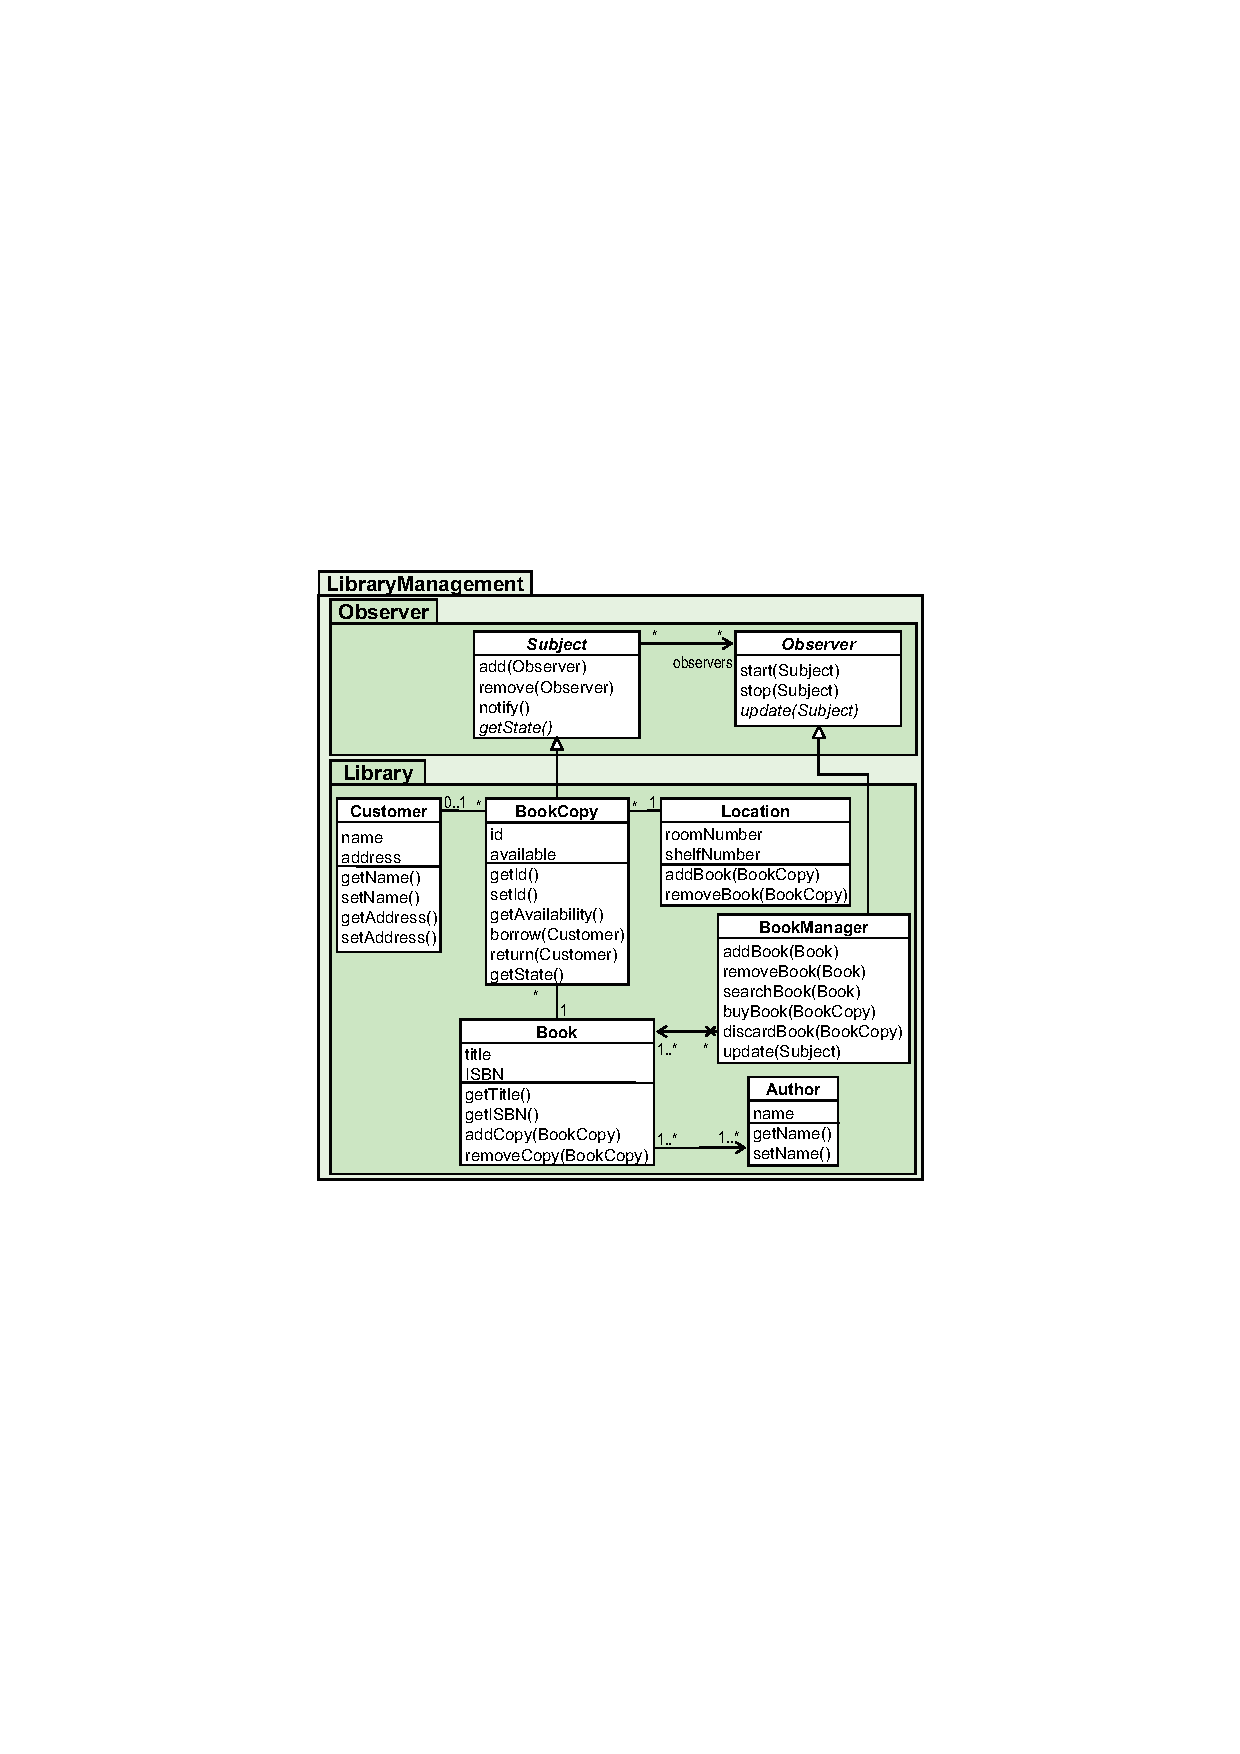
\includegraphics[width=0.4\linewidth]{figures/figure1}
	\caption{xxx (Quelle zitieren, wenn nicht selbst erstellt)}
	\label{fig:xxx}
\end{figure}
Tabellen
Jede Tabelle muss im Fließtext referenziertw werden. Für Tabellen gelten die selben Regeln, wie für Abbildungen (siehe dazu Abschnitt \ref{sec:abbildungen}).

Eine Beispiel einer Tabelle ist in Tabelle \ref{tab:xxx} zu finden:
\begin{table}
	\centering
	\begin{tabular}{| >{\bfseries}l | c | r | }
		\hline
			\rowcolor{orange} \bfseries Linksbündig & \bfseries Zentriert & \bfseries Rechtsbündig \\
		\hline
		\hline
			Zeile 1 & xxx & xxx \\\hline
			Zeile 2 & xxx & \dots \\\hline
			\multirow{2}{*}{Zeile3}
			& xxx & xxx \\\cline{2-3}
			& xxx & xxx \\\hline
		\hline
			\multicolumn{3}{| c |}{xxx} \\\hline
	\end{tabular}
	\caption{xxx (Quelle angeben)}
	\label{tab:xxx}
\end{table}

Bitte beachten Sie, dass Tabellen generell so einfach wie möglich gehalten werden sollen. Tabelle \ref{tab:xxx} dient unter anderem dazu Studierenden zu zeigen, wie Tabellen in \LaTeX\xspace erstellt werden können und wie Farben verwendet werden.
_____________________________


In diesem Kapitel wird die eigentliche Problemlösung in einem oder mehreren Unterkapiteln ausgeführt. Die Strukturierung dieser Kapitel ist naturgemäß sehr stark von der konkreten Aufgabenstellung abhängig. Der Name dieses Kapitels ist anzupassen, z.B. Umfeldbeschreibung -- Fallbeispiel \dots, konkreter schreiben je nach Art Diplomarbeit/Fragestellung.
\makeatletter\ifthesis@masterthesis
Nachfolgend einige Beispiele für unterschiedliche Arten von Diplomarbeiten.

Bei einer Software-Entwicklungsarbeit bieten sich folgende Unterkapitel an:
\begin{itemize}
	\item Im Kapitel \enquote{Design} sollte die konzeptionelle Lösung vorgestellt, diskutiert und begründet werden. Das Ergebnis dieses Kapitels könnte beispielsweise eine Protokoll-Architektur sein.
	\item Im Kapitel \enquote{Modelle} erfolgt üblicherweise das Feindesign. In diesem Kapitel könnten beispielsweise einzelne Protokolle bzw. Algorithmen aus der vorher definierten Protokoll-Architektur eingeführt und diskutiert werden. Achtung: Generell darauf achten, bei der eingangs erläuterten Notation zu bleiben und nicht Synonyme zu verwenden, verwirrt den Leser.
	\item Das Kapitel \enquote{Implementierung} sollte sich dann vorwiegend mit den Details der Umsetzung befassen. In diesem Kapitel sollte nur im Ausnahmefall exemplarisch Quellcode vorgesehen werden. Vielmehr sollten alle Probleme, die bei der Realisierung aufgetreten sind, dokumentiert, interpretiert und die Lösung erläutert werden.
\end{itemize}

Bei einer Arbeit zu einem abstrakteren Thema, bei dem ein oder mehrere Fallbeispiele aus der industriellen Praxis bearbeitet werden, bieten sich folgende Unterkapitel an:
\begin{itemize}
	\item Im Unterkapitel \enquote{Analyse der Problemstellung} wird die konkrete Problemstellung (die Situation im betrachteten Unternehmen) der Fallbeispiele beschrieben. Das Ergebnis dieses Kapitels könnte eine schematische Netzwerk- oder Applikationsarchitektur sein.
	\item Im Unterkapitel \enquote{Fallbeispiel} sollte sich (analog zur Implementierung in der Software-Entwicklung) mit den konkreten Details der Umsetzung befassen. Hier wird dargelegt, wie das zuvor identifizierte Lösungsschema konkret zur Anwendung gelangen kann bzw. welche Probleme während des Umsetzungsprojekts aufgetreten sind.
\end{itemize}

Bei einer Arbeit, deren Grundlage eine Auswahl eines Softwaresystems ist, bieten sich folgende Unterkapitel an:
\begin{itemize}
	\item IST-Analyse
	\item Hardware und Softwareausstattung
	\item Beschreibung der Geschäftsprozesse
	\item Schwachstellenanalyse des Unternehmens
	\item SOLL-Konzeption
	\item Auswahlverfahren möglicher verfügbarer Systeme -- Kriterienkatalog
	\item Einführung des neuen Systems
\end{itemize}

Bei einer Arbeit, deren Fokus auf der Durchführung und Auswertung von Fragebögen liegt, bieten sich folgende Unterkapitel an:
\begin{itemize}
	\item Im Kapitel \enquote{Problemstellung und Fragebogendesign} wird die fachliche Problemstellung detailliert erläutert und der Inhalt des Fragebogens in Bezug zur Problemstellung dargestellt.
	\item Im Kapitel \enquote{Befragungsmethode} werden die Untersuchungsobjekte (z.B. Praktische Ärzte), die Grundgesamtheit (Anzahl praktische Ärzte in Venezuela), Stichprobengesamtheit und das Verfahren zur Stichprobenziehung und das Erhebungsverfahren (Verteilung und Rücklauf der Fragebögen) beschrieben.
	\item Im Kapitel \enquote{Auswertungsmethode} werden die möglichen Auswertungsmethoden aufgelistet und ggf. begründet die ausgewählte Methode beschrieben.
	\item Im Kapitel \enquote{Befragungsdurchführung} wird die Untersuchungsdurchführung (z.B. Zeit, Ort der Befragung, Zeitraum der gesamten Befragung, besondere für das Untersuchungsergebnis oder zukünftige Forschungsarbeiten relevante Vorkommnisse etc.) dargestellt.
\end{itemize}

Hier intensive Rücksprache mit Ihren jeweiligen Fachbetreuern halten, mehrere Diplomarbeiten der Fakultät zu diesem Themenbereich durchsehen. Unabhängig vom Typ der Diplomarbeit werden im nachfolgenden Kapitel die konkreten Ergebnisse beschrieben.